\section{Pianificazione}
Sulla base delle cadenza fissate in §1.6, la ripartizione delle attività di progetto avviene tramite:
\begin{itemize}
\item \textbf{Analisi};
\item \textbf{Consolidamento requisiti};
\item \textbf{Progettazione e codifica per la Technology Baseline};
\item \textbf{Progettazione di dettaglio e codifica};
\item \textbf{Validazione e collaudo}.
\end{itemize}  

\subsection{Analisi}
\textit{Periodo: da 2020-03-16 a 2020-04-13} \\
La fase di analisi è suddivisa nel seguente modo:
\begin{itemize}
\item \textbf{Identificazione degli strumenti}: attività rivolta a determinare gli strumenti da utilizzare per le comunicazioni, stesura dei documenti, versionamento, sviluppo e verifica del sistema;
\item \textbf{Norme di Progetto}: sono l'insieme delle regole da seguire per lo svolgimento dei processi e la realizzazione del prodotto. Il documento \textit{Norme di Progetto}, è redatto dall'\textit{Amministratore};
\item \textbf{Studio di Fattibilità}: attività svolta dagli \textit{Analisti} con lo scopo di analizzare i capitolati, in linea generale, per stabilire quale di essi sia una proposta realizzabile. Inoltre è un'attività propedeutica all'\textit{Analisi dei Requisiti};
\item \textbf{Analisi dei Requisiti}: sulla base dell'attività precedente, vengono identificati e definiti i requisiti del sistema. Come per il documento \textit{Studio di Fattibilità}, anche \textit{Analisi dei Requisiti}, viene redatto dagli \textit{Analisti};
\item \textbf{Piano di Qualifica}: attività dell'\textit{Amministratore} e del \textit{Progettista} che si occupa di stabilire le metodologie per garantire la qualità del prodotto. In particolar modo la seconda figura si focalizza sulla parte programmatica;
\item \textbf{Piano di Progetto}: il lavoro da svolgere viene suddiviso in compiti, risorse e attività da parte del \textit{Responsabile}, che ha anche il compito di calcolare il preventivo di periodo del progetto. Il tutto viene riportato sempre da parte del \textit{Responsabile} nel documento \textit{Piano di Progetto};
\item \textbf{Glossario}: tutti i vocaboli di difficile interpretazione vengono individuati riportati nel documento \textit{Glossario}.
\end{itemize}

\begin{figure}[H]
\centering
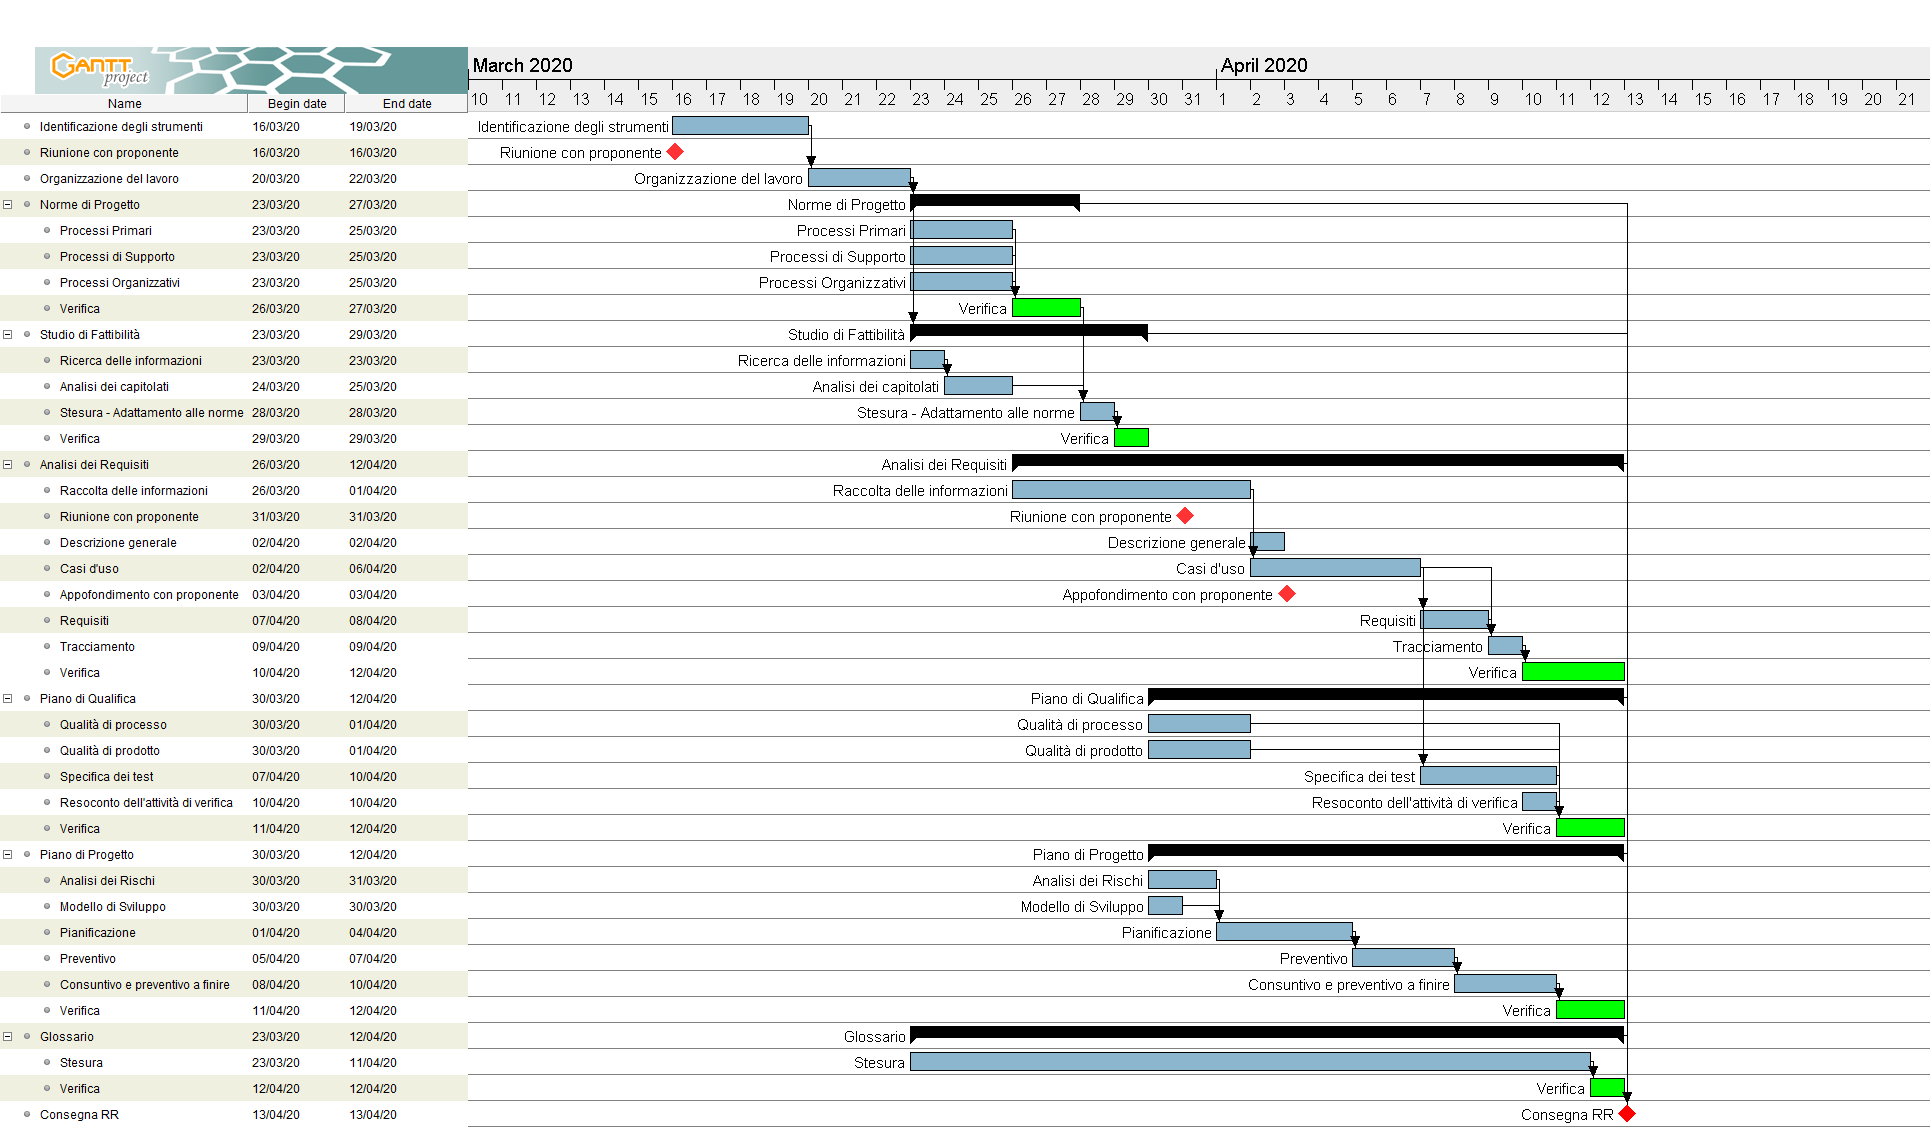
\includegraphics[scale=0.24]{./img/gantt/analisi.png}
\caption{Diagramma di Gantt della fase di Analisi}
\end{figure}

\subsection{Consolidamento dei requisiti}
\textit{Periodo: da 2020-04-14 a 2020-04-20}\\
La fase di consolidamento è così suddivisa:
\begin{itemize}
\item \textbf{Approfondimento personale}: attività intenta a fissare ed approfondire le informazioni riguardanti i requisiti evidenziati nella precedente fase;
\item \textbf{Raccolta informazioni}: raccolta delle informazioni necessarie per la presentazione;
\item \textbf{Stesura presentazione}: preparazione del materiale necessario alla presentazione del 2020-04-20;
\item \textbf{Studio personale}: tempo dedicato ai membri del gruppo, per studiare le informazioni contenute nella presentazione.
\end{itemize}

\begin{figure}[H]
\centering
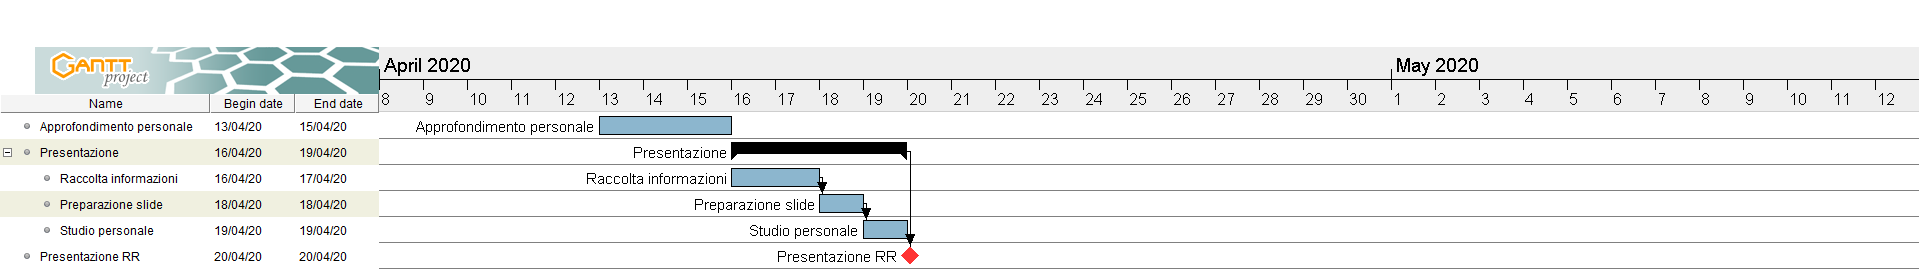
\includegraphics[scale=0.24]{./img/gantt/consolidamento_requisiti.png}
\caption{Diagramma di Gantt della fase di Consolidamento dei requisiti}
\end{figure}

\subsection{Progettazione e codifica per la Technology Baseline}
\textit{Periodo: da 2020-04-21 a 2020-05-11}\\
Questa fase coincide con il giorno successivo alla presentazione del 2020-04-20 e termina con la consegna del materiale per la \textbf{Revisone di Progettazione}. La fase è così suddivisa in:
\begin{itemize}
\item \textbf{Incrementi e verifica}: sulla base dei feedback del committente e del proponente, viene migliorato e verificato il materiale del precedente rilascio.
\item \textbf{Technology Baseline}: vengono identificati i design pattern\glo necessari allo sviluppo del sistema e verranno riportati nell'allegato tecnico insieme al tracciamento dei requisiti. Inoltre viene presentato, al committente e al proponente, un prototipo per mezzo di un repository\glo. In questo periodo saranno implementati solo una parte di requisiti, ovvero quelli che ricoprono le funzionalità di base. Successivamente verranno raffinati i requisiti già implementati, se non completi, e saranno implementate le funzionalità che permetteranno di soddisfare tutti i requisiti. Per fare ciò sono stati individuati i seguenti incrementi:
	\begin{itemize}
		\item \textbf{Incremento 1: ottenimento file JSON:} verrà implementata una pagina web per ottenere il file JSON, mediante l'uso della libreria di React;
		\item \textbf{Incremento 2: caricamento file JSON:} verrà implementata la funzionalità per l'inserimento nel plugin del file JSON, contenente i predittori. Verrà usato React in sinergia con gli strumenti di sviluppo di plugin offerti dalla piattaforma Grafana;
		\item \textbf{Incremento 3: collegamento al flusso dati:} verrà implementata la funzione di collegamento del plugin ad un flusso di dati;
	\end{itemize}
\end{itemize}

\begin{figure}[H]
\centering
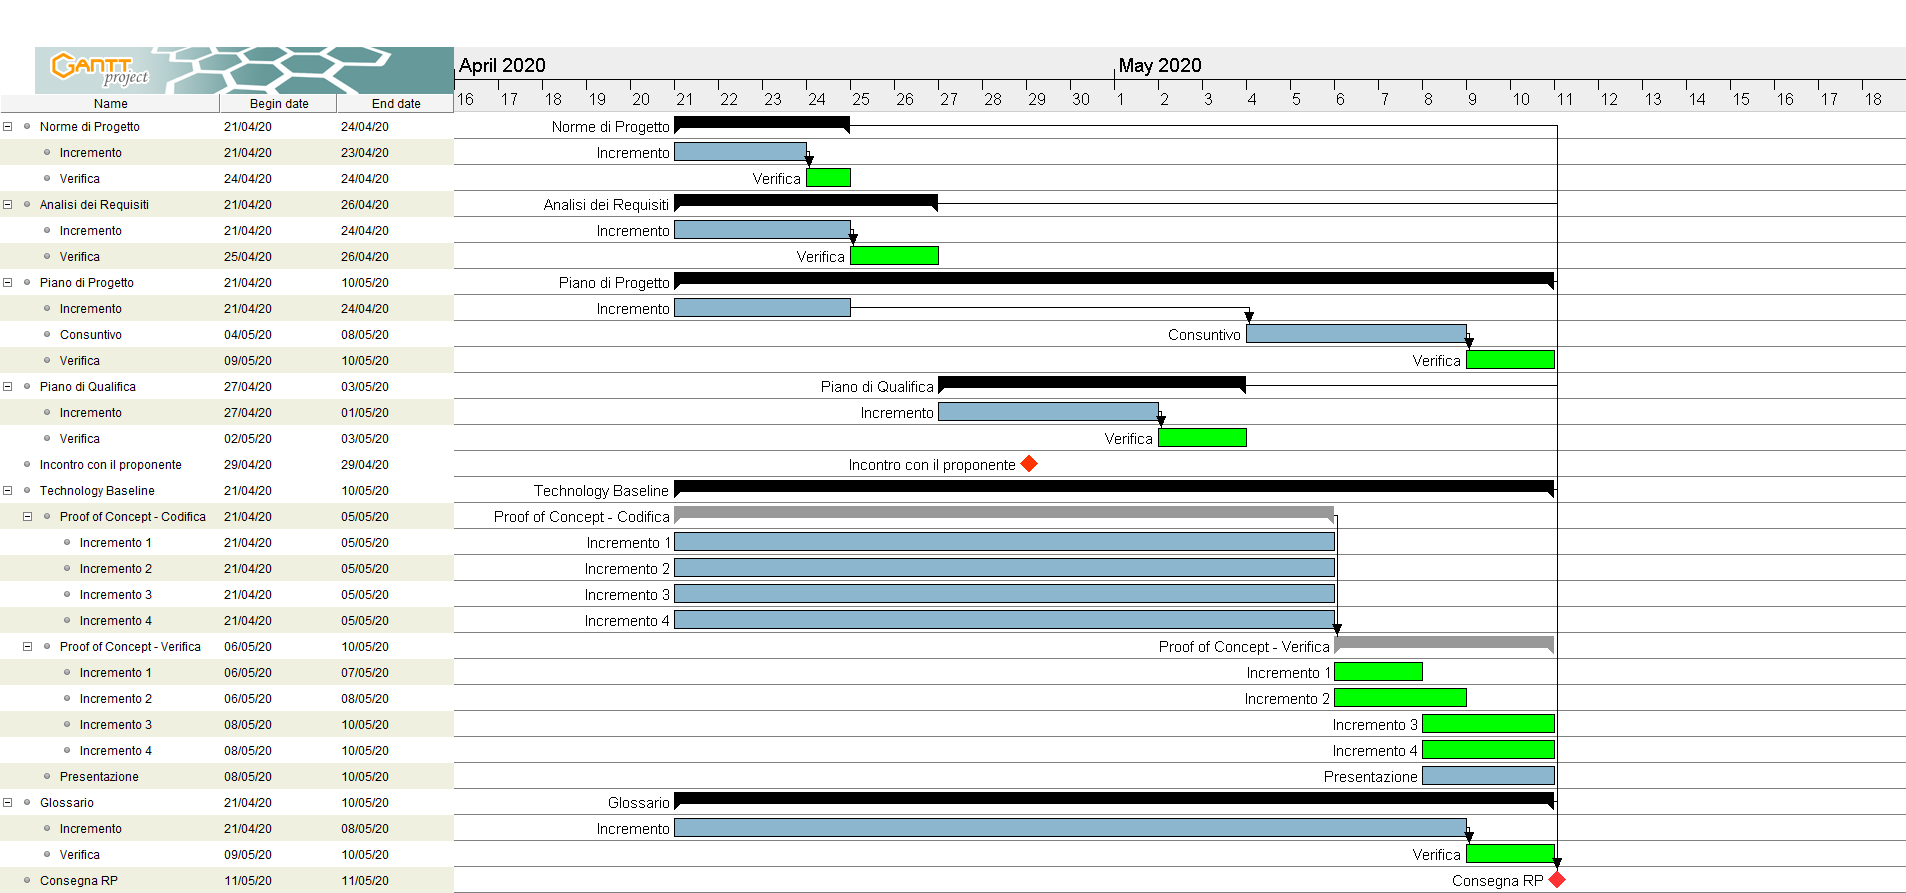
\includegraphics[scale=0.24]{./img/gantt/progettazione_architetturale.png}
\caption{Diagramma di Gantt della fase di Progettazione e codifica per la Technology Baseline}
\end{figure}

\subsection{Progettazine di dettaglio e codifica}
\textit{Periodo: da 2020-05-11 a 2020-06-11}\\
Questa fase è compresa tra il giorno successivo alla presentazione del 2020-05-11 e la consegna della \textit{Revisione di Qualifica}.
\begin{itemize}
\item \textbf{Product Baseline}: le singole unità di cui è composta l'architettura definita nella \textit{Technology Baseline}, vengono ulteriormente analizzate;
\item \textbf{Incrementi e verifica}: sulla base dei feedback del committente e del proponente, viene migliorato e verificato il materiale del precedente rilascio.
\end{itemize}

\begin{figure}[H]
\centering
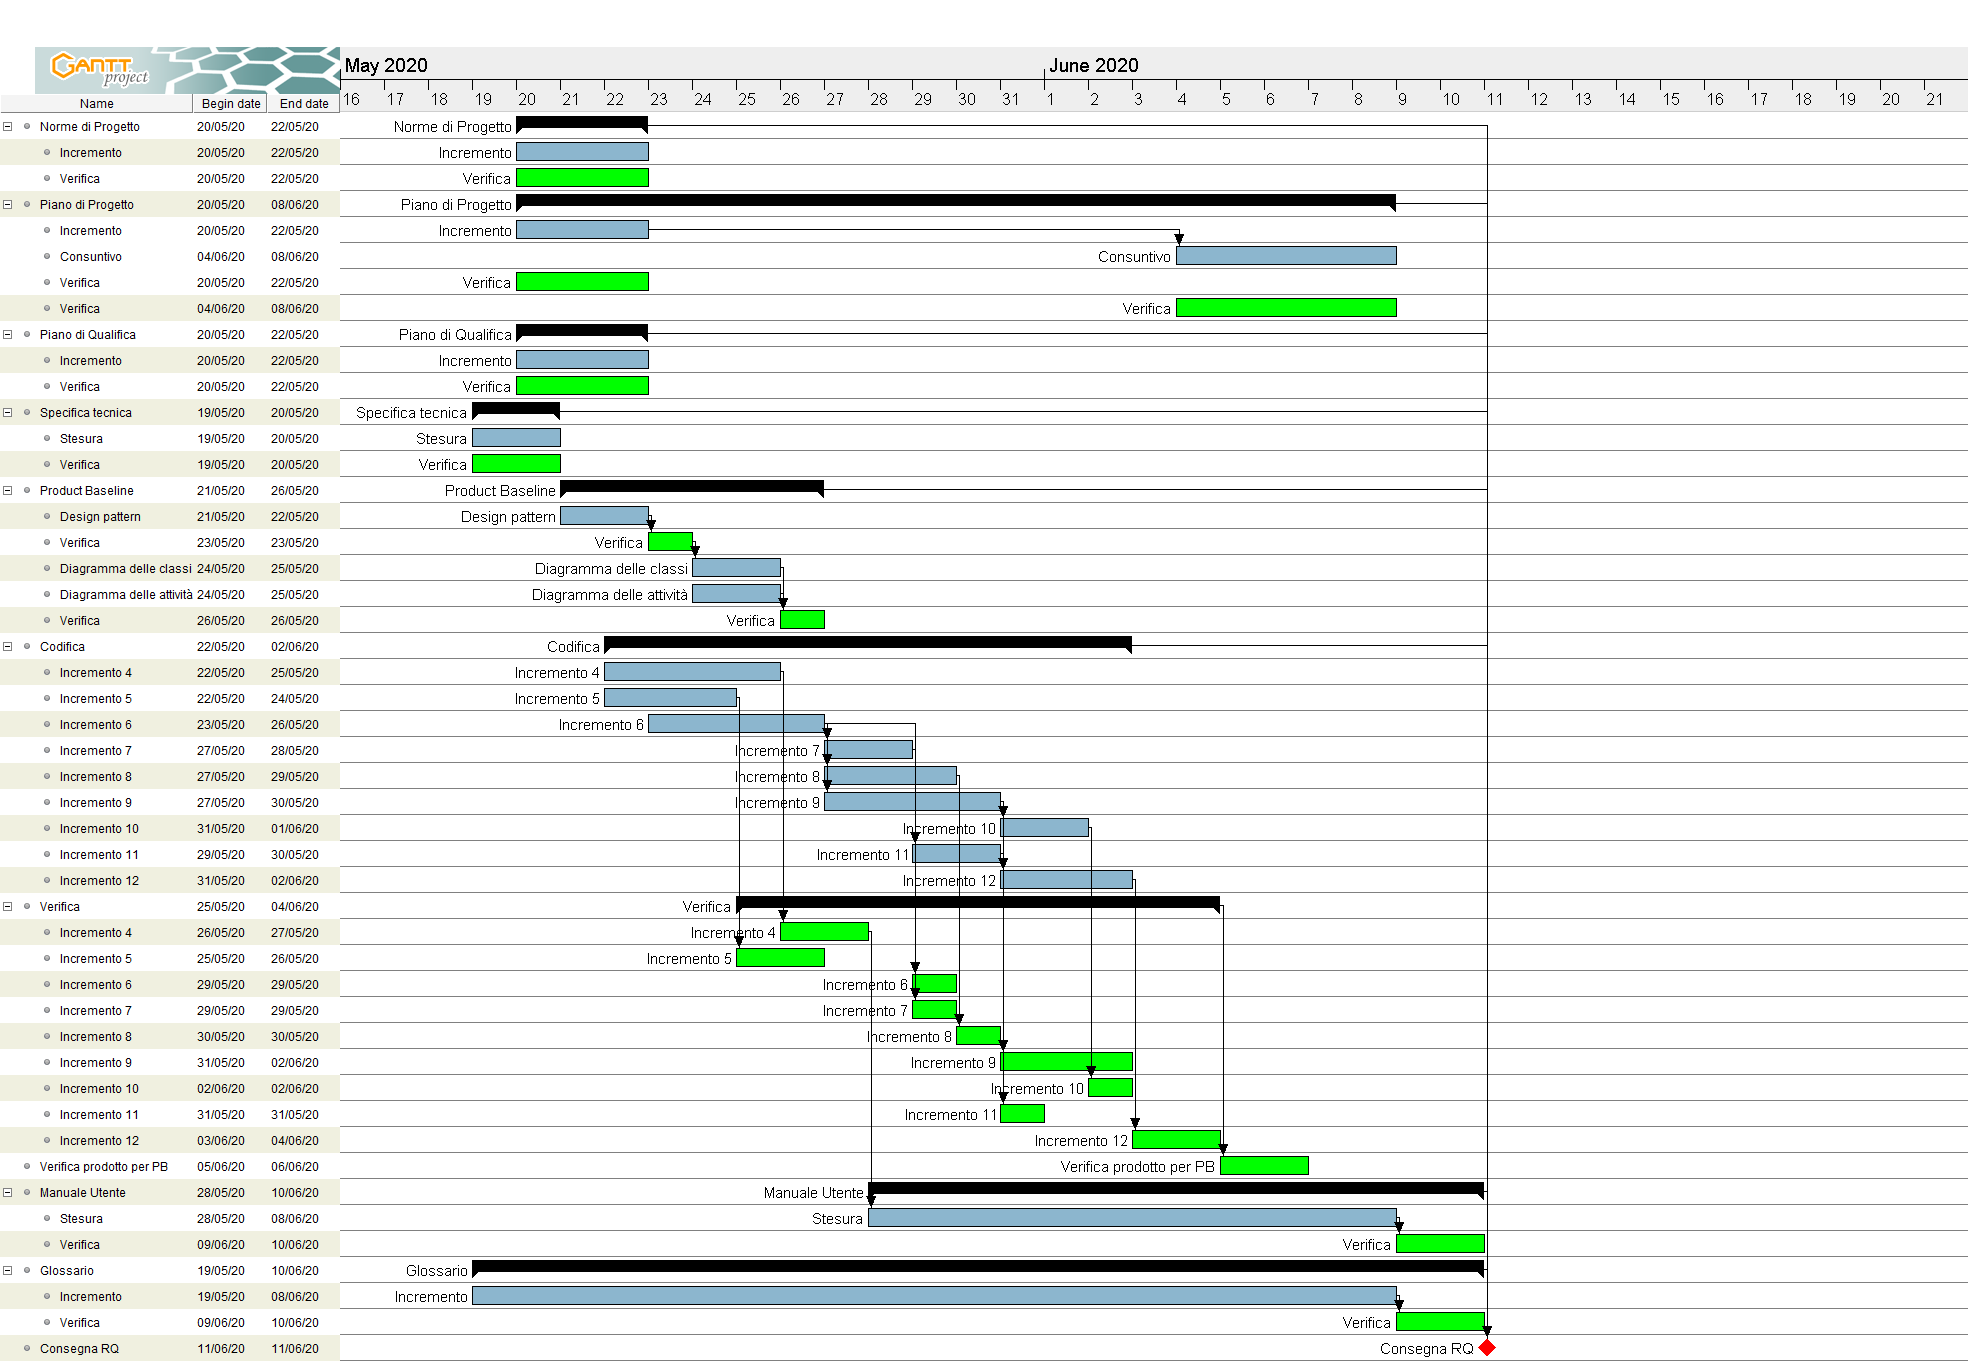
\includegraphics[scale=0.24]{./img/gantt/progettazione_dettaglio_codifica.png}
\caption{Diagramma di Gantt della fase di Progettazione di dettaglio e codifica}
\end{figure}

\subsection{Validazione e collaudo}
\textit{Periodo: da 2020-06-19 a 2020-07-06}\\
La seguente fase inizia il giorno seguente la \textit{Revisione di Qualifica} e termina con la consegna del materiale richiesto per la \textit{Revisione di Avanzamento}.
\begin{itemize}
\item \textbf{Incremento}: nel caso risultasse necessario vengono effettuati miglioramenti sulla base di feedback;
\item \textbf{Validazione e collaudo}: la validazione effettua test sul prodotto, me tre la convalidazione controlla se viene rispettata la coerenza tra il prodotto e le specifiche evidenziate nel documento \textit{Analisi dei Requisiti};
\item \textbf{Manuale Sviluppatore}: viene redatto il documento \textit{Manuale dello Sviluppatore}, il quale conterrà le informazioni necessarie allo sviluppo, mantenimento e manutenzione del prodotto;
\item \textbf{Manuale Utente}: viene redatto il documento \textit{Manuale dell'Utente}, il quale conterrà le informazioni necessarie all'utilizzo del prodotto.
\end{itemize}

\begin{figure}[H]
\centering
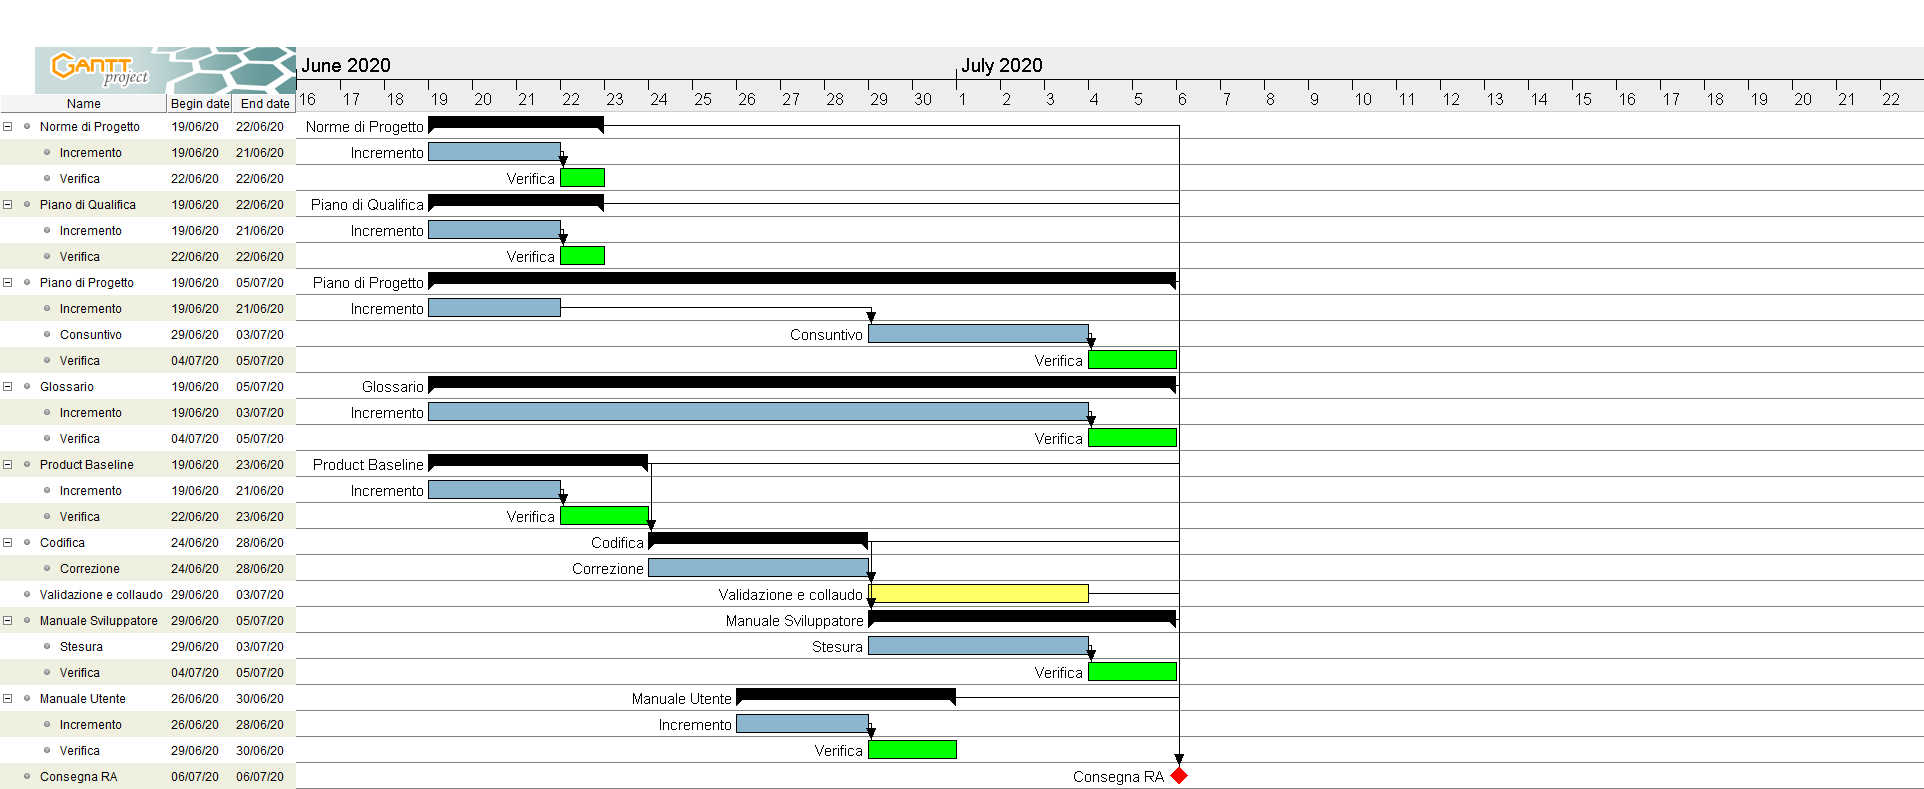
\includegraphics[scale=0.24]{./img/gantt/validazione_collaudo.png}
\caption{Diagramma di Gantt della fase di Validazione e collaudo}
\end{figure}